\documentclass[11pt, oneside]{article}   	% use "amsart" instead of "article" for AMSLaTeX format
\usepackage{geometry}                		% See geometry.pdf to learn the layout options. There are lots.
\geometry{letterpaper}                   		% ... or a4paper or a5paper or ... 
%\geometry{landscape}                		% Activate for rotated page geometry
%\usepackage[parfill]{parskip}    		% Activate to begin paragraphs with an empty line rather than an indent
\usepackage{graphicx}				% Use pdf, png, jpg, or eps§ with pdflatex; use eps in DVI mode
								% TeX will automatically convert eps --> pdf in pdflatex		
\usepackage{amssymb}
\usepackage{amsmath}
\usepackage{float}
%SetFonts
\usepackage{tikz}
\usetikzlibrary{shapes.misc,shapes.geometric,arrows.meta,positioning,shadows.blur,chains,scopes}
\tikzstyle{startstop} = [rectangle, rounded corners, minimum width=3cm, minimum height=1cm, draw=black, fill=blue!16]
\tikzstyle{io} = [trapezium, trapezium left angle=70, trapezium right angle=110, minimum width=3cm, minimum height=1cm, text centered, draw=black, fill=blue!30]
\tikzstyle{process} = [rectangle, minimum width=3cm, minimum height=1cm, text centered, draw=black, fill=orange!30]
\tikzstyle{decision} = [diamond, minimum width=3cm, minimum height=1cm, text centered, draw=black, fill=green!30]
\usetikzlibrary{shapes.geometric, arrows}
\tikzstyle{arrow} = [thick,->,>=stealth]
\usepackage{ragged2e}
\usepackage{adjustbox}
\usepackage{blindtext}
\usepackage[utf8]{inputenc}
\newcommand{\Var}{\operatorname{Var}}
% Default fixed font does not support bold face
\DeclareFixedFont{\ttb}{T1}{txtt}{bx}{n}{12} % for bold
\DeclareFixedFont{\ttm}{T1}{txtt}{m}{n}{12}  % for normal

% Custom colors
\usepackage{color}
\definecolor{deepblue}{rgb}{0,0,0.5}
\definecolor{deepred}{rgb}{0.6,0,0}
\definecolor{deepgreen}{rgb}{0,0.5,0}

\usepackage{listings}
\usepackage{smartdiagram}

\makeatletter
\NewDocumentCommand{\smartdiagramx}{r[] m}{%
    \StrCut{#1}{:}\diagramtype\option
    \IfStrEq{\diagramtype}{priority descriptive diagram}{% true-priority descriptive diagram
        \pgfmathparse{subtract(\sm@core@priorityarrowwidth,\sm@core@priorityarrowheadextend)}
        \pgfmathsetmacro\sm@core@priorityticksize{\pgfmathresult/2}
        \pgfmathsetmacro\arrowtickxshift{(\sm@core@priorityarrowwidth-\sm@core@priorityticksize)/2}
        \begin{tikzpicture}[every node/.style={align=center,let hypenation}]
        \foreach \smitem [count=\xi] in {#2}{\global\let\maxsmitem\xi}
        \foreach \smitem [count=\xi] in {#2}{%
            \edef\col{\@nameuse{color@\xi}}
            \node[description,drop shadow](module\xi)
            at (0,0+\xi*\sm@core@descriptiveitemsysep) {\smitem};
            \draw[line width=\sm@core@prioritytick,\col]
            ([xshift=-\arrowtickxshift pt]module\xi.base west)--
            ($([xshift=-\arrowtickxshift pt]module\xi.base west)-(\sm@core@priorityticksize pt,0)$);
        }%
        \coordinate (A) at (module1);
        \coordinate (B) at (module\maxsmitem);
        \CalcHeight(A,B){heightmodules}
        \pgfmathadd{\heightmodules}{\sm@core@priorityarrowheightadvance}
        \pgfmathsetmacro{\distancemodules}{\pgfmathresult}
        \pgfmathsetmacro\arrowxshift{\sm@core@priorityarrowwidth/2}
        \begin{pgfonlayer}{background}
        \node[priority arrow,rotate=180,transform shape] at ([xshift=-\arrowxshift pt]module\maxsmitem.north west){};
        \end{pgfonlayer}
        \end{tikzpicture}
    }{}% end-priority descriptive diagram
}%

\makeatother



% Python style for highlighting
\newcommand\pythonstyle{\lstset{
language=Python,
basicstyle=\ttm,
otherkeywords={self},             % Add keywords here
keywordstyle=\ttb\color{deepblue},
emph={MyClass,__init__},          % Custom highlighting
emphstyle=\ttb\color{deepred},    % Custom highlighting style
stringstyle=\color{deepgreen},
frame=tb,                         % Any extra options here
showstringspaces=false            % 
}}


% Python environment
\lstnewenvironment{python}[1][]
{
\pythonstyle
\lstset{#1}
}
{}

% Python for external files
\newcommand\pythonexternal[2][]{{
\pythonstyle
\lstinputlisting[#1]{#2}}}

% Python for inline
\newcommand\pythoninline[1]{{\pythonstyle\lstinline!#1!}}

\title{A proposed solution architecture for the application of anomaly detection in predictive maintenance}
\author{Yapi Donatien Achou}
%\date{}							% Activate to display a given date or no date

\begin{document}
\maketitle

\section{Introduction}
Predictive maintenance  for machines and industrial equipments can be defined as a maintenance philosophy or more generally a framework with a set of methods used to predict and prevent machine failure in order to avoid unexpected downtime and reduce related human and financial cost. 
\justify
As a framework, predictive maintenance has 4 levels. In level 1, visual inspection of machines or equipments are performed in order to assess any damage.
In addition, equipment must fail before they are replaced, which can incur a high production cost. In level 2 and 3, machines characteristics such as vibration, temperature, electrical current, voltage etc are monitored continually or periodically depending on their criticality. This is called condition monitoring. In condition monitoring, the goal is to detect any change in machine normal behaviour, in order to detect failure as early as possible and schedule maintenance accordantly. Maintenance actions are performed periodically regardless of machine health condition. In level 4, big data and machine learning are the main driving forces in detecting failure and planning maintenance. At this level, maintenance action are not performed periodically but are planned according to machine health condition derived from the application of anomaly detection techniques. This reduce unnecessary maintenance action and significantly cuts down maintenance cost as well as increasing machine life time.
\justify
According to PriceWaterhouseCoopers (PWC), one of the four largest auditing and consulting company in the world,  a survey from 280 companies in Belgium, Germany and the Nederland, revealed that only 
$11 \%$ of companies have reached level 4 \cite{pwc}. The application of level 4 requires collecting, saving and analysing large amount of data, from which maintenance decision can be made. Anomaly detection methods and more generally supervised and unsupervised learning techniques are used in the analysis phase.
\justify
In this report we outline part of the components of the solution architecture for a successful application of level 4. 

\subsection{The solution architecture}
Industrial equipments and machines operate under varying conditions, load and requirements. This suggest that the systems are very dynamic in nature and any solution architecture for anomaly detection must be dynamic and adaptive, to say the least. To achieve a dynamic and successful anomaly detection procedure there are three necessary and iterative stages/requirements that must be fulfilled. 
These stages/requirements are conveniently named as upstream, midstream and downstream stage.
\justify
%%%%%%%%%%%%%%%%%%%%%%%%%%%%%%%%%%%%%%%%%%%%%%%%%%%
% picture goes here 
\begin{center}
\smartdiagramx[priority descriptive diagram]{
    \textbf{Downstream stage}\\ 
    \begin{itemize}
    \item Data driven modelling
    \end{itemize}
    ,
    \textbf{Midstream stage}
    \begin{itemize}
    \item Conceptual modelling
    \end{itemize},
   \textbf{Upstream stage}
   \begin{itemize}
    \item Data collection
    \end{itemize}
   }
   \end{center}
   
\justify
In the upstream stage the data and the metadata are collected. In this stage, often the main focus is on the data, which is collected and stored in a database. Nonetheless more attention should also be placed on the metadata. By metadata we mean all informations about the data as well as any maintenance activity performed on the system. The latter is crucially important for reasons that will be outline shortly. 
\justify
The midstream stage consists of designing a conceptual model for the whole system.
In this stage FMECA or Failure mode, effects and criticality analysis is performed and different data attributes are map to each components of the system. This is done in order to thoroughly understand the system and latter apply appropriate anomaly detection techniques.
\justify
lastly in the downstream stage, the anomaly detection techniques are carefully chosen based on the conceptual model designed in the midstream stage. In the next three sections we describe each stage and stress they importance relative to each other and relative to the whole problem of anomaly detection.

\section{Upstream stage}
Most company moving into stage four of the predictive maintenance framework have been collecting data for a period of time. The data is often collected automatically and logged continuously to a database or data warehouse/data platform. In addition, various information regarding the data are also logged. These information are called metadata. They include detailed description of the data, the name of each time series attribute, the maintenance log, to name a few. 

\begin{figure}[H] %  figure placement: here, top, bottom, or page
   \centering
   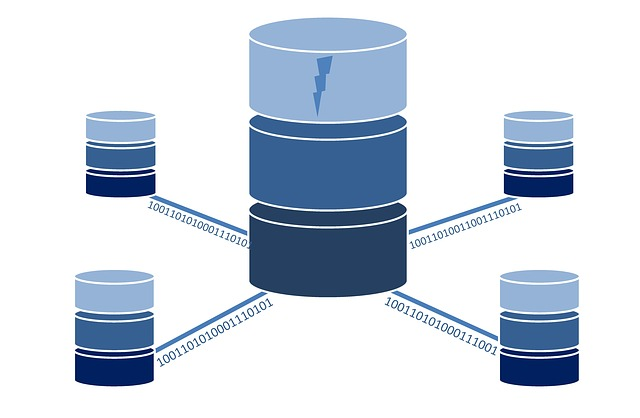
\includegraphics[width=4in]{database.jpg} 
   \caption{Picture representation of the data collection process}
   \label{fig:db}
\end{figure}
\justify
The maintenance log are as important as the time series data. By maintenance log we mean any maintenance activities that have been performed on a machine or system of machines. This includes the exact date, the detailed description of activity performed and the findings if any. The maintenance log will later be used for cross referencing with the time series. By cross referencing we mean the used of the maintenance log to detect a variation in the probability distribution of the data.
\justify
Often most companies use excel sheets that are saved locally to log maintenance activities. The downside of this is that the sheets often lack informations as they can be field after the maintenance activities have been performed. In addition, they can not directly be used to auto train an anomaly detection model which has been deployed on a production environment. To mitigate this problem,
We suggest that the sheet be replaced by a web application which is accessible on an iPad device like. This way the maintenance activity can be filed in as the maintenance activity are being performed and the maintenance log can be directly push to a database. Let look at a scenario where this can be relevant.
\justify
Suppose that a machine learning model has been trained base on the past five years data. This training data probability distribution is generated by a machine. Assume now that few pieces of that machine have been replaced one year later. We have no guaranty that the probability distribution upon which our model has been build is the same. However, with an automatic maintenance log system such as a web application, an automatic training procedure can be triggered when maintenance activity are logged into the database. Thus we create an automatic triggered base learning or self learning model based on maintenance activities. This will help maintain the integrity of the model.

\section{Midstream stage}
The midstream stage consists of building a conceptual model of the system of machine or machine. The conceptual model is the representation of the system. It allows a better understanding of the system. It is import for a successful development of a data driven model. This stage is a multi disciplinary stage where domain expert and data scientist should work closely to describe and understand the system. Procedure such as Failure Mode Effect and Criticality Analysis or FMECA must be performed to 
\begin{itemize}
\item Describe the system as a block diagram
\item list failure modes and severity of failure
\item list cause and effect of each failure mode.
\end{itemize} 
\justify
\begin{figure}[H]
\begin{center}
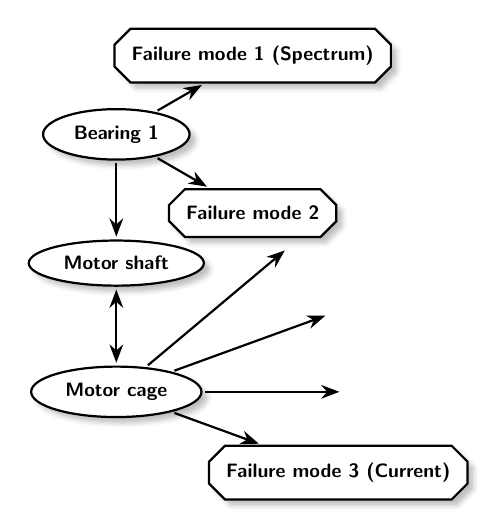
\begin{tikzpicture}
  [
    ->,
    >=Stealth,
    shorten >=1pt,
    shorten <=1pt,
    thick,
    main node/.style={fill=white, draw, font=\sffamily\scriptsize\bfseries, blur shadow, align=center},
    hex/.style={main node, chamfered rectangle},
    ell/.style={main node, ellipse},
    blur shadow={shadow opacity=25},
    start chain=main going below,
  ]
  \node [on chain, ell] {Bearing 1};
  {[start branch=limits up going {at=(\tikzchainprevious), shift=(30:2)}]
    \node [on chain, hex, join=by ->] {Failure mode 1 (Spectrum)};
  }
  {[start branch=limits up going {at=(\tikzchainprevious), shift=(-30:2)}]
    \node [on chain, hex, join=by ->] {Failure mode 2};
  }
  \node [on chain, ell, join=by {->}] {Motor shaft};
  \node [on chain, ell, join=by <->] {Motor cage};
  {[start branch=ep going {at=(main-3), shift=({60-(\tikzchaincount-1)*20}:3)}, every on chain/.append style={join={with main-3 by ->}}]
    \node [on chain] {};
    \node [on chain] {};
    \node [on chain] {};
    \node [on chain, hex] {Failure mode 3 (Current)};
    %\node [on chain, hex] {Failure mode 4 (voltage)};
  }
\end{tikzpicture}
\caption{Illustration of an hypothetical conceptual model}
\label{fig:conceptual}
\end{center}
\end{figure}
\justify
Figure \ref{fig:conceptual} shows an hypothetical conceptual mode. In this model the system is reduced to a motor with a shaft, a cage and one bearing. the double arrow between the motor shaft and the motor cage indicates that they is a direct interaction between the two parts. The failure mode of each part is also indicated.
\justify
In addition, time series attributes must be map with each part of the system. For example in Figure \ref{fig:conceptual}, the envelop spectrum is needed to detect failure mode 1 while current is required to detect failure mode 3. A detail conceptual model can therefore facilitate the data driven modelling where the actual anomaly detection or other statistical/machine learning modelling are performed.
\clearpage
\section{Downstream stage}
After a thorough understanding and analysis of the system, a system of anomaly detection strategies can be derived. This stage is concerned with the machine learning/statistical model training and building. Most of the time we are dealing with time series. Therefore time series analysis as well as supervised and unsupervised methods are applied.
\begin{figure}[H] %  figure placement: here, top, bottom, or page
   \centering
   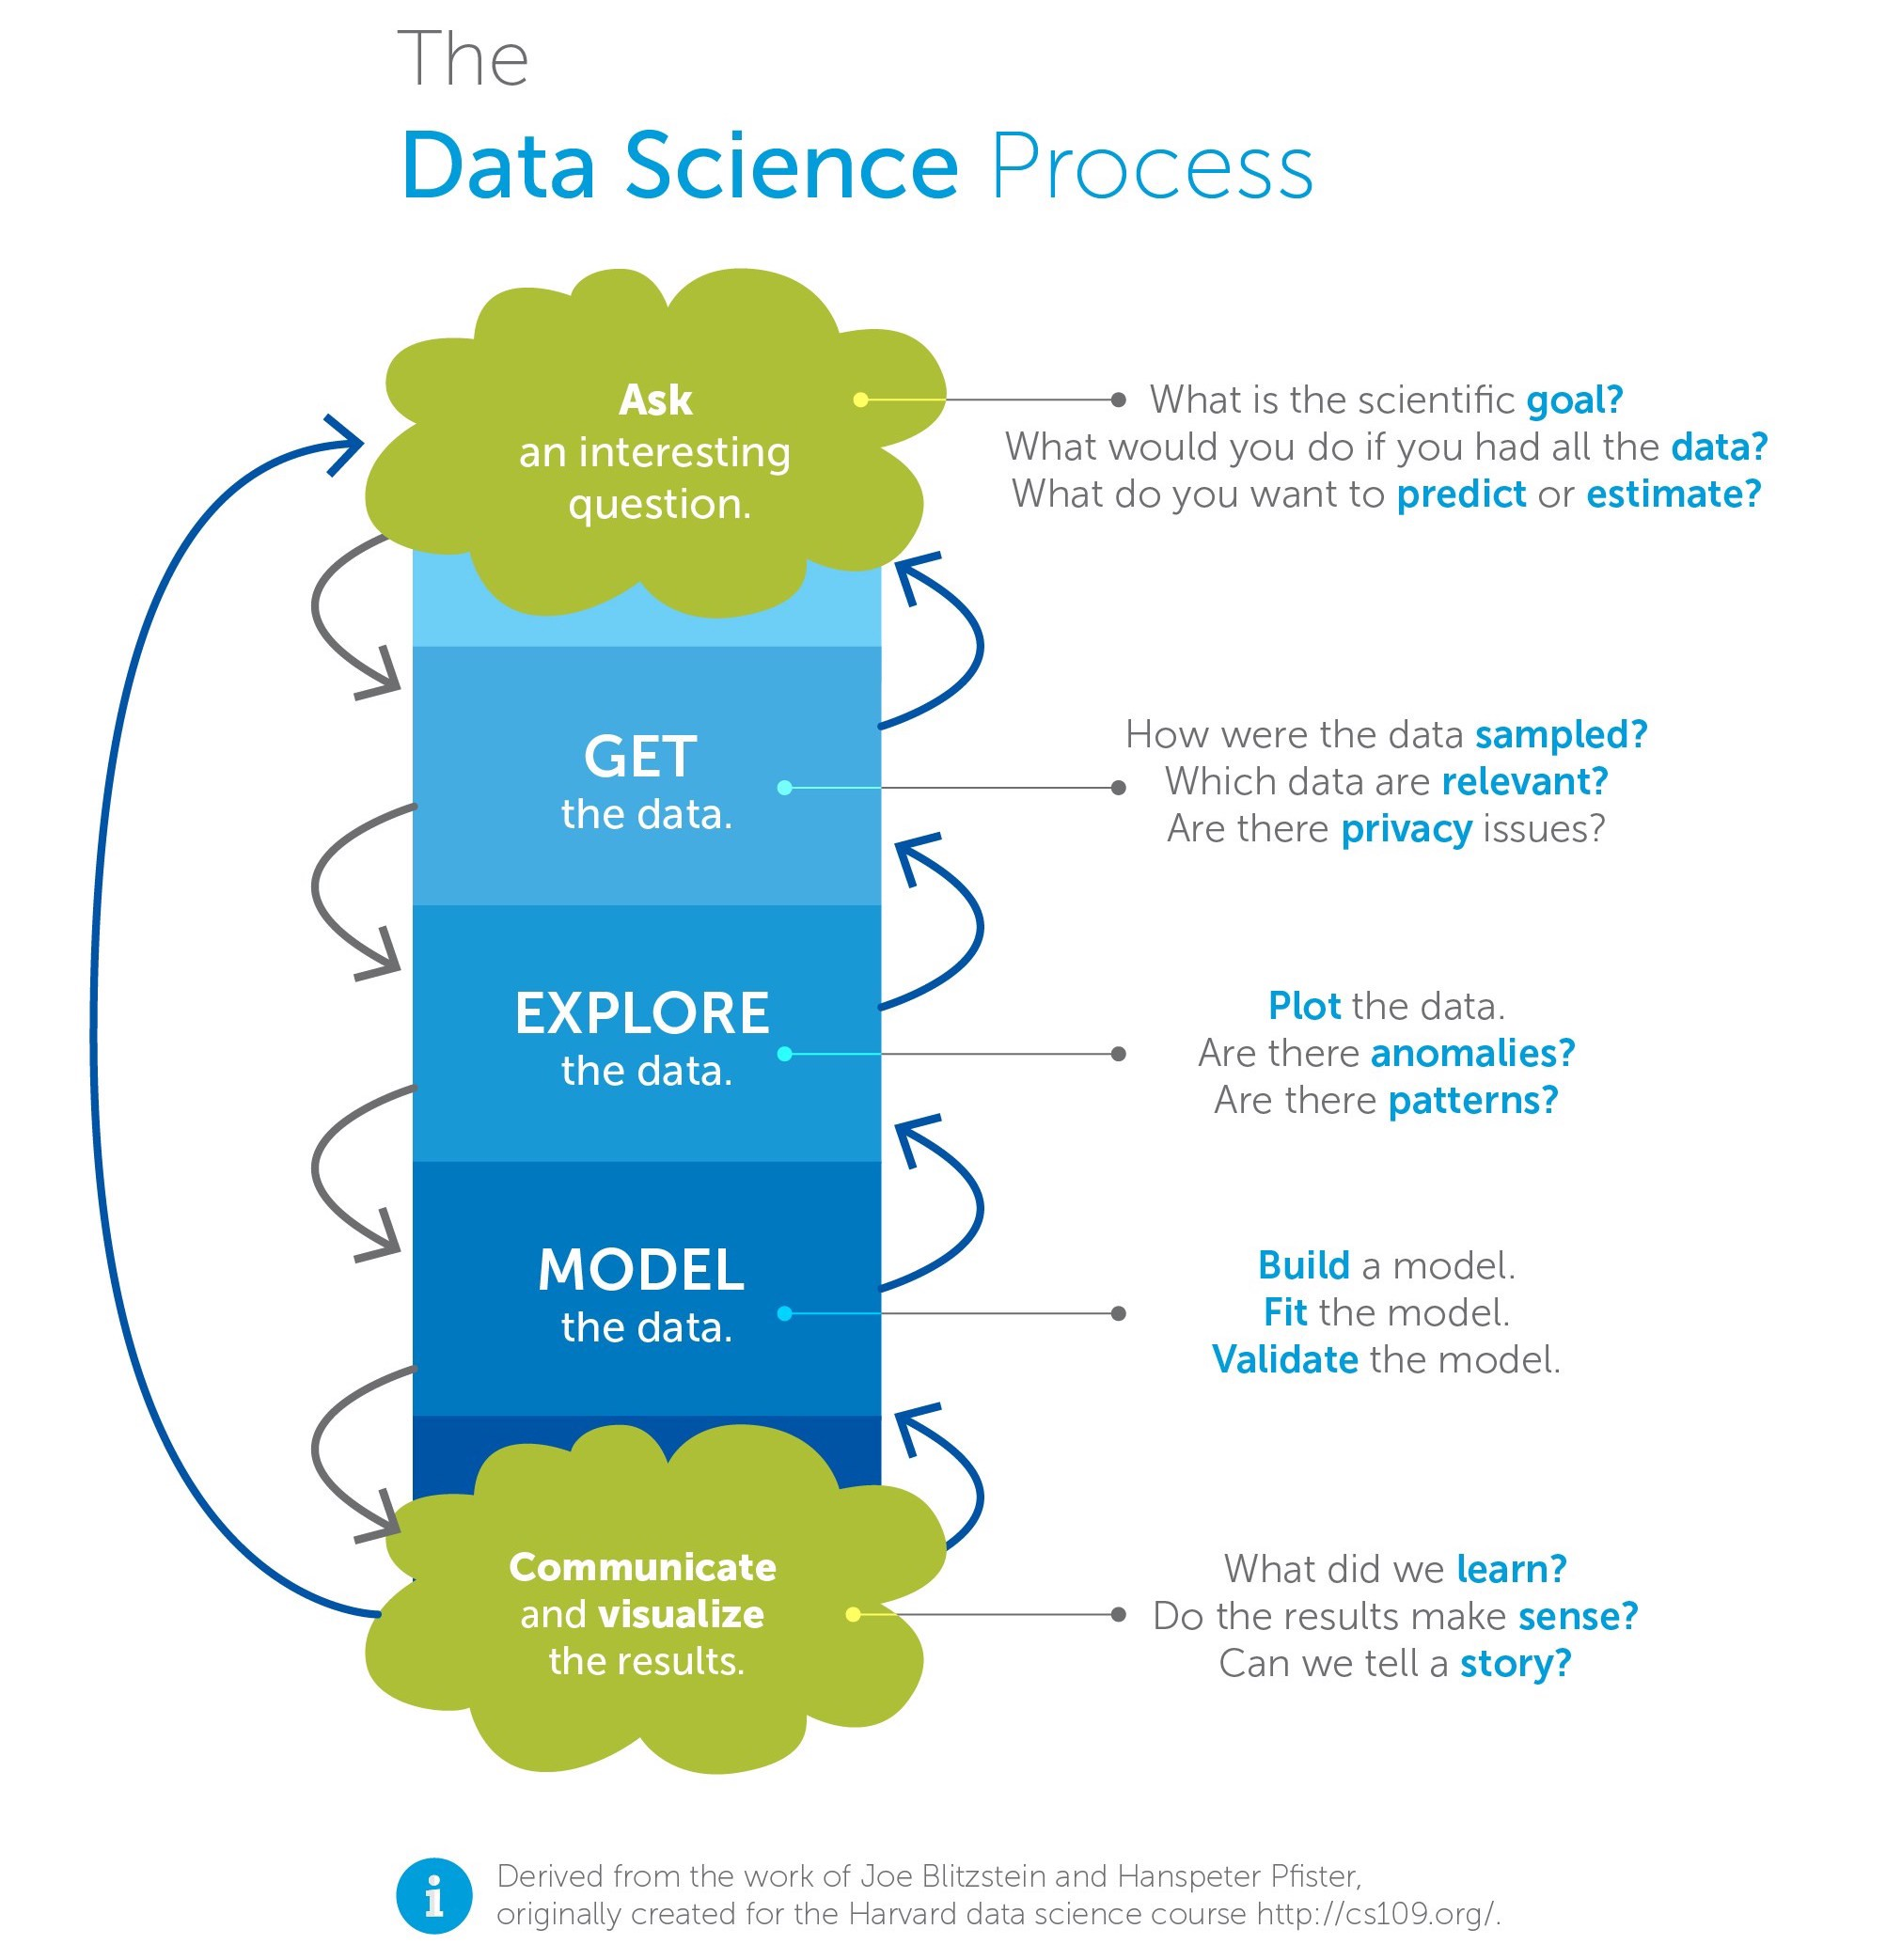
\includegraphics[width=5in]{dprocess.jpeg} 
   \caption{An illustration of the data science process}
   \label{fig:dp}
\end{figure}

\section{Conclusion}










\begin{thebibliography}{9}

%\bibitem{norden2008} 
%Norden E. Huang and Zhaohua Wu 
%\textit{A review on Hilbert-Huang Transform: Methods and its Application to Geophysical Studies}. 
%Review of Geophysics, 2008
% 
%\bibitem{norden1998} 
%Norden E. Huang, Zheng Shen, Steven R. Long, Manlic C. Wu, Hsing H.Shih, Quanan Zheng, Nai-Chyuan Yen, Chi Chao Tung and Henry H. Liu
%\textit{The Empirical mode decomposition and the Hilbert Spectrum for nonlinear and non-stationary time series analysis}
%Proc. R. Soc. Lond. A (1998) 455, 903:995.
%
%\bibitem{chandola} 
%Varun Chandola, Arindam Banerjee, and Vipin Kumar.
%\textit{Anomaly detection: A survey}
%Proc. R. Soc. Lond. A (1998) 455, 903:995.


 
\bibitem{pwc} 
Michel Mulders and Mark Haarman
\textit{Predictive maintenance 4.0. Predict the unpredictable, June 2017}

 
%\bibitem{hui2007} 
%Hui Li, Yuping Zhang and Haiqi Zheng
%\textit{Hilbert-Huang transform and marginal spectrum for detecting and diagnosis of localized defects in roller bearings}
%Journal of Mechanical Technology, 2007

\end{thebibliography}


\end{document}  